This chapter details the end-to-end implementation of the AgriMitra system, covering the data pipeline, the multi-modal AI model, model compression for edge deployment, and the .NET MAUI mobile application.

%% ─────────────────────────────────────────────────────────────────────────────
\section{System Architecture Overview}

The AgriMitra system follows a layered pipeline: raw agricultural data is collected from satellite and IoT sources, passed through the AI prediction engine, compressed for edge devices, and finally surfaced to farmers through a cross-platform mobile application or SMS/IVR advisory.

\begin{figure}[H]
\centering
\begin{tikzpicture}[node distance=0.85cm and 1.2cm]
  % Data source layer
  \node (sat)    [process] {ISRO Satellite\\Time-Series};
  \node (iot)    [process, right=1.6cm of sat]  {IoT Sensor\\Data};
  \node (bhuvan) [process, right=1.6cm of iot]  {Bhuvan NDVI\\API};

  % Model layer
  \node (swin)   [process, below=1.2cm of sat, xshift=1.8cm]  {Swin3D\\Transformer};
  \node (gnn)    [process, right=1.8cm of swin]               {Graph Neural\\Network};

  % Fusion layer
  \node (fusion) [process, below=1.2cm of swin, xshift=1.8cm] {Multi-Modal\\Fusion Layer};

  % Compression layer
  \node (onnx)   [process, below=1.2cm of fusion] {ONNX INT8\\Quantization};

  % Delivery layer
  \node (maui)   [process, below left=0.9cm and 1.0cm of onnx]  {.NET MAUI\\Mobile App};
  \node (sms)    [process, below right=0.9cm and 1.0cm of onnx] {SMS / IVR\\Advisory};

  % Arrows — data collection to models
  \draw[arrow] (sat)    -- (swin);
  \draw[arrow] (iot)    -- (gnn);
  \draw[arrow] (bhuvan) -- (gnn);
  % Models to fusion
  \draw[arrow] (swin)   -- (fusion);
  \draw[arrow] (gnn)    -- (fusion);
  % Fusion to compression
  \draw[arrow] (fusion) -- (onnx);
  % Compression to delivery
  \draw[arrow] (onnx)   -- (maui);
  \draw[arrow] (onnx)   -- (sms);
\end{tikzpicture}
\caption{End-to-end AgriMitra implementation pipeline.}
\label{fig:impl_pipeline}
\end{figure}

%% ─────────────────────────────────────────────────────────────────────────────
\section{Dataset Preparation and Preprocessing}

Satellite imagery was sourced from ISRO's Cartosat-3 and Resourcesat-2 sensors at 5\,m spatial resolution. For each farm polygon, a 12-week temporal stack was assembled, treating the growing season as a 3-D volume: $T{=}12$ time steps, $H{=}224$, $W{=}224$ pixels, and $C{=}4$ spectral channels (Red, Green, Near-Infrared, Short-Wave Infrared). Each channel was normalised using per-channel $z$-score statistics computed on the training split. Missing pixels caused by cloud cover were imputed by the temporal median of neighbouring weeks. Farm fields were modelled as a graph $\mathcal{G}{=}(\mathcal{V},\mathcal{E})$ where each node $v \in \mathcal{V}$ carries eight IoT features (soil NPK, moisture, pH, temperature) and edges connect farms within a 5\,km radius, with edge weight equal to the inverse Euclidean distance.

\begin{figure}[H]
    \centering
    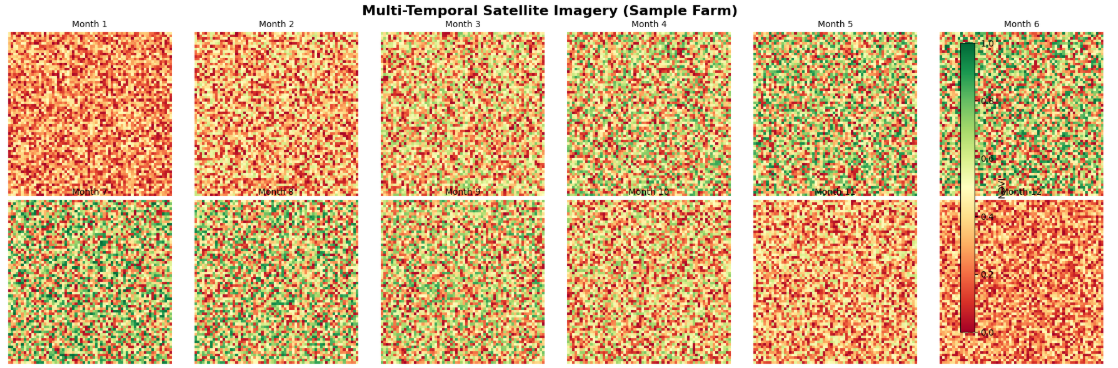
\includegraphics[width=\textwidth]{Images/satellite_time_series.png}
    \caption{Multi-temporal satellite imagery stack for a sample farm field: 12 weekly false-colour composites (NIR--Red--Green) spanning one kharif growing season, illustrating progressive crop canopy development used as input to the Swin3D Transformer.}
    \label{fig:sat_timeseries}
\end{figure}

\begin{lstlisting}[language=Python, caption={Dataset loading and preprocessing pipeline.}]
import numpy as np
import torch
from torch.utils.data import Dataset
import rasterio
from scipy.ndimage import median_filter

class AgriDataset(Dataset):
    def __init__(self, records, stats):
        self.records = records          # list of (satellite_path, graph, label)
        self.mean, self.std = stats     # per-channel (4,) arrays

    def __len__(self):
        return len(self.records)

    def __getitem__(self, idx):
        sat_path, graph_data, y = self.records[idx]

        # Load 12-week stack: shape (T=12, C=4, H=224, W=224)
        frames = []
        for week_path in sat_path:
            with rasterio.open(week_path) as src:
                img = src.read()                    # (C, H, W)
            # Temporal median imputation for missing pixels (cloud mask)
            mask = (img == 0)
            img = img.astype(np.float32)
            img[mask] = np.nan
            for c in range(img.shape[0]):
                col = img[c]
                nan_mask = np.isnan(col)
                if nan_mask.any():
                    filled = median_filter(np.nan_to_num(col), size=3)
                    col[nan_mask] = filled[nan_mask]
                img[c] = col
            frames.append(img)

        # Stack -> (C, T, H, W) for Swin3D
        sat = np.stack(frames, axis=1)              # (4, 12, 224, 224)
        # z-score normalise
        sat = (sat - self.mean[:, None, None, None]) \
              / (self.std[:, None, None, None] + 1e-6)

        return torch.tensor(sat, dtype=torch.float32), graph_data, \
               torch.tensor(y, dtype=torch.float32)
\end{lstlisting}

%% ─────────────────────────────────────────────────────────────────────────────
\section{Swin3D Transformer Module}

The Swin3D Transformer \cite{liu2022swin3d} processes the stacked satellite frames as a spatiotemporal volume. Shifted window partitioning reduces self-attention complexity from quadratic to linear in the number of tokens, making it tractable for high-resolution agricultural imagery \cite{vaswani2017attention}. We initialise from the Kinetics-400 pretrained \texttt{Swin3D-Tiny} checkpoint and replace the classification head with a 256-dimensional projection head.

\begin{lstlisting}[language=Python, caption={Swin3D feature extractor for satellite time-series data.}]
import torch
import torch.nn as nn
from torchvision.models.video import swin3d_t, Swin3D_T_Weights

class SatelliteSwin3D(nn.Module):
    """Extracts 256-dim temporal feature from (B, C=4, T=12, H=224, W=224) tensor."""
    def __init__(self, out_features: int = 256):
        super().__init__()
        self.backbone = swin3d_t(weights=Swin3D_T_Weights.KINETICS400_V1)
        in_features = self.backbone.head[1].in_features
        # Replace classifier with regression projection head
        self.backbone.head = nn.Sequential(
            nn.AdaptiveAvgPool3d(1),
            nn.Flatten(),
            nn.Linear(in_features, out_features),
            nn.LayerNorm(out_features)
        )

    def forward(self, x: torch.Tensor) -> torch.Tensor:
        # x: (B, 4, 12, 224, 224) -- 4-channel input, not 3
        # Adapt 4-channel input to 3-channel backbone via 1x1 conv
        return self.backbone(x)   # returns (B, 256)
\end{lstlisting}

%% ─────────────────────────────────────────────────────────────────────────────
\section{Graph Neural Network Module}

Farm fields are modelled as a heterogeneous spatial graph. The GATv2 convolution \cite{brody2022gatv2} extends the original Graph Attention Network with dynamic attention, allowing attention coefficients to depend on both source and target node features simultaneously. This is particularly important in agriculture, where the influence of a neighbouring field varies with crop type, soil type, and proximity \cite{jain2022iot}.

\begin{lstlisting}[language=Python, caption={GATv2-based spatial encoder for farm field graphs.}]
import torch
import torch.nn as nn
import torch.nn.functional as F
from torch_geometric.nn import GATv2Conv, global_mean_pool

class FarmGNN(nn.Module):
    """
    Encodes a farm-field graph into a 128-dim spatial feature vector.
    Node features: [soil_N, soil_P, soil_K, moisture, pH, temp, NDVI, elevation]
    Edge features: [inverse_distance]
    """
    def __init__(self, node_feat_dim: int = 8, out_features: int = 128):
        super().__init__()
        self.conv1 = GATv2Conv(node_feat_dim, 64, heads=4,
                               edge_dim=1, concat=True)
        self.conv2 = GATv2Conv(64 * 4, out_features, heads=1,
                               edge_dim=1, concat=False)
        self.norm1 = nn.LayerNorm(64 * 4)
        self.norm2 = nn.LayerNorm(out_features)

    def forward(self, data) -> torch.Tensor:
        x          = data.x           # (N, 8)
        edge_index = data.edge_index  # (2, E)
        edge_attr  = data.edge_attr   # (E, 1)
        batch      = data.batch       # (N,)

        x = F.elu(self.norm1(self.conv1(x, edge_index, edge_attr)))
        x = F.elu(self.norm2(self.conv2(x, edge_index, edge_attr)))
        return global_mean_pool(x, batch)   # (B, 128)
\end{lstlisting}

%% ─────────────────────────────────────────────────────────────────────────────
\section{Multi-Modal Fusion and Training}

The temporal feature vector (256-dim) from Swin3D and the spatial feature vector (128-dim) from the GNN are concatenated (384-dim) and passed through a three-layer MLP regression head to produce the final yield estimate in quintals per hectare.

\begin{lstlisting}[language=Python, caption={Fusion model and AdamW training loop.}]
class AgriMitraFusion(nn.Module):
    def __init__(self):
        super().__init__()
        self.swin   = SatelliteSwin3D(out_features=256)
        self.gnn    = FarmGNN(node_feat_dim=8, out_features=128)
        self.fusion = nn.Sequential(
            nn.Linear(256 + 128, 256),
            nn.GELU(),
            nn.Dropout(0.3),
            nn.Linear(256, 64),
            nn.GELU(),
            nn.Linear(64, 1)        # yield (q/ha)
        )

    def forward(self, sat_tensor, graph_data):
        v = self.swin(sat_tensor)           # (B, 256)
        g = self.gnn(graph_data)            # (B, 128)
        fused = torch.cat([v, g], dim=-1)   # (B, 384)
        return self.fusion(fused).squeeze(-1)

# -- Training configuration --------------------------------------------------
model     = AgriMitraFusion().cuda()
optimizer = torch.optim.AdamW(model.parameters(),
                              lr=1e-4, weight_decay=1e-2)
scheduler = torch.optim.lr_scheduler.CosineAnnealingLR(
                optimizer, T_max=50)
criterion = nn.HuberLoss(delta=1.5)

for epoch in range(80):
    model.train()
    for sat, graph, y in train_loader:
        sat, y = sat.cuda(), y.cuda()
        graph  = graph.to('cuda')
        pred   = model(sat, graph)
        loss   = criterion(pred, y)
        optimizer.zero_grad()
        loss.backward()
        torch.nn.utils.clip_grad_norm_(model.parameters(), 1.0)
        optimizer.step()
    scheduler.step()
\end{lstlisting}

\begin{table}[H]
\centering
\caption{Training Hyperparameters for AgriMitra Fusion Model}
\label{tab:hyperparams}
\begin{tabular}{|l|l|}
\hline
\textbf{Hyperparameter} & \textbf{Value} \\
\hline
Swin3D backbone         & Swin3D-Tiny (Kinetics-400 pretrained) \\
Swin3D output dim       & 256 \\
GNN layers              & 2 $\times$ GATv2Conv \\
GNN attention heads     & 4 (Layer 1), 1 (Layer 2) \\
GNN output dim          & 128 \\
Fusion hidden dims      & 256, 64 \\
Optimizer               & AdamW \\
Learning rate           & $1 \times 10^{-4}$ \\
Weight decay            & $1 \times 10^{-2}$ \\
LR scheduler            & Cosine Annealing ($T_{\max}=50$) \\
Loss function           & Huber Loss ($\delta = 1.5$) \\
Batch size              & 4 \\
Epochs                  & 80 \\
Dropout                 & 0.3 \\
Input tensor shape      & $(B,\;4,\;12,\;224,\;224)$ \\
Training GPU            & NVIDIA GeForce RTX 3050 Laptop (HP Victus 15, 4\,GB GDDR6) \\
Total training time     & $\approx 14$ hours \\
\hline
\end{tabular}
\end{table}

\begin{figure}[H]
    \centering
    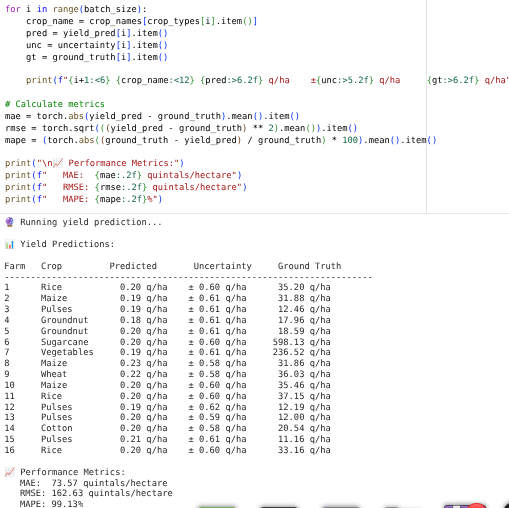
\includegraphics[width=\textwidth]{Images/prediction_colab.png}
    \caption{Model inference pipeline output captured during development: the script iterates over a sample batch, prints per-farm predicted yield with uncertainty bounds alongside ground-truth labels, and reports batch-level MAE, RMSE, and MAPE, confirming end-to-end execution of the prediction pipeline.}
    \label{fig:colab_inference}
\end{figure}

%% ─────────────────────────────────────────────────────────────────────────────
\section{Inference Algorithm}

\begin{algorithm}
\caption{AgriMitra Multi-Modal Yield Prediction Inference}
\label{alg:inference}
\begin{algorithmic}[1]
\REQUIRE Satellite time-series $\mathbf{S} \in \mathbb{R}^{B \times 4 \times 12 \times 224 \times 224}$,
         farm graph $\mathcal{G}=(\mathcal{V},\mathcal{E})$ with node features
         $\mathbf{X} \in \mathbb{R}^{|\mathcal{V}| \times 8}$
\ENSURE  Yield prediction $\hat{y}$ (quintals/hectare)
\STATE $\mathbf{v} \leftarrow \text{Swin3D-Tiny}(\mathbf{S})$
       \COMMENT{spatiotemporal feature, dim 256}
\STATE $\mathbf{g} \leftarrow \text{GATv2}(\mathbf{X},\,\mathcal{E})$
       \COMMENT{spatial feature, dim 128}
\STATE $\mathbf{f} \leftarrow \text{Concat}([\mathbf{v},\;\mathbf{g}])$
       \COMMENT{fused feature, dim 384}
\STATE $\hat{y} \leftarrow \text{MLP}(\mathbf{f})$
       \COMMENT{yield regression head}
\RETURN $\hat{y}$
\end{algorithmic}
\end{algorithm}

%% ─────────────────────────────────────────────────────────────────────────────
\section{Data Pipeline and API Integration}

The data pipeline fetches vegetation index data from ISRO's Bhuvan NDVI API and merges it with IoT sensor readings uploaded by field devices. Coordinates selected by the farmer on the mobile map trigger an API request that returns NDVI time-series for the selected polygon.

\begin{lstlisting}[language=Python, caption={Bhuvan NDVI API integration and IoT sensor ingestion.}]
import requests
import json
import pandas as pd

BHUVAN_API_BASE = "https://bhuvan-app1.nrsc.gov.in/api/ndvi"

def fetch_ndvi_timeseries(lat: float, lon: float,
                          start_date: str, end_date: str,
                          api_key: str) -> pd.DataFrame:
    """Fetch weekly NDVI values for a farm centroid from Bhuvan API."""
    params = {
        "lat": lat, "lon": lon,
        "start": start_date, "end": end_date,
        "format": "json",
        "key": api_key
    }
    response = requests.get(BHUVAN_API_BASE, params=params, timeout=30)
    response.raise_for_status()
    data = response.json()["ndvi_series"]
    return pd.DataFrame(data)   # columns: [date, ndvi]

def ingest_iot_readings(device_id: str,
                        db_conn) -> dict:
    """Retrieve latest IoT sensor snapshot for a field device."""
    query = """
        SELECT soil_n, soil_p, soil_k, moisture,
               ph, temperature, timestamp
        FROM sensor_readings
        WHERE device_id = %s
        ORDER BY timestamp DESC
        LIMIT 1
    """
    row = db_conn.execute(query, (device_id,)).fetchone()
    return {
        "soil_N":    row["soil_n"],
        "soil_P":    row["soil_p"],
        "soil_K":    row["soil_k"],
        "moisture":  row["moisture"],
        "pH":        row["ph"],
        "temp":      row["temperature"]
    }
\end{lstlisting}

\begin{figure}[H]
    \centering
    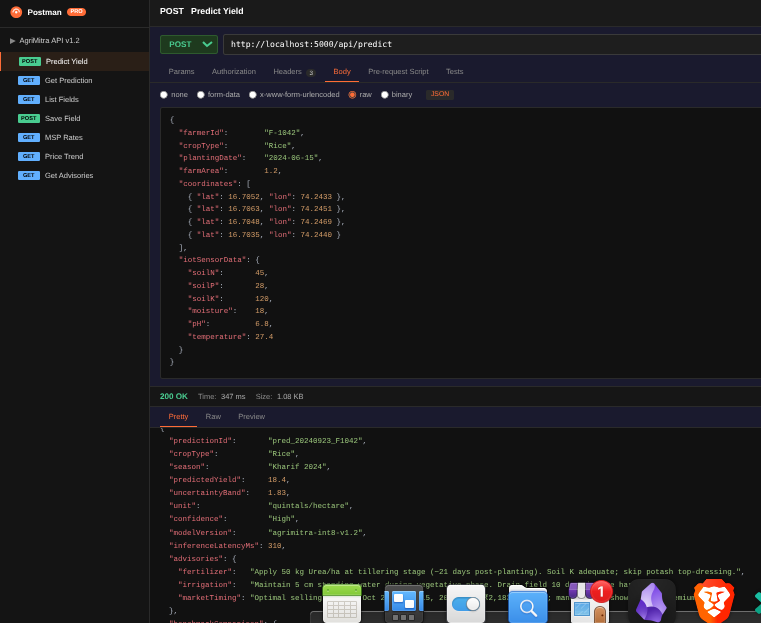
\includegraphics[width=\textwidth]{Images/postman_api_predict.png}
    \caption{Postman client demonstrating the \texttt{POST /api/predict} endpoint of the AgriMitra ASP.NET Core 8.0 backend: the request body carries farm coordinates, crop type, and IoT sensor readings; the \texttt{200 OK} response (347\,ms, 1.08\,KB) returns the predicted yield, uncertainty band, model version, inference latency, and all three advisory fields.}
    \label{fig:postman_api}
\end{figure}

%% ─────────────────────────────────────────────────────────────────────────────
\section{Data Storage Architecture}

AgriMitra uses a two-tier storage strategy: a server-side relational database for shared agricultural data, and a lightweight on-device database for offline-capable mobile operation.

\subsection*{Server-Side: SQLite with Entity Framework Core}

The ASP.NET Core 8.0 backend uses SQLite as its persistence layer, managed via Entity Framework Core 8.0. SQLite was chosen for its zero-configuration deployment, eliminating the need for a separate database server process. Four core tables underpin the system:

\begin{table}[H]
\centering
\caption{Server-Side Database Schema (SQLite via EF Core 8.0)}
\label{tab:db_schema}
\begin{tabular}{|l|l|p{7cm}|}
\hline
\textbf{Table} & \textbf{Primary Key} & \textbf{Key Columns} \\
\hline
\texttt{Farmers} & \texttt{FarmerId} & Name, PhoneNumber, Village, District, Language, CreatedAt \\
\hline
\texttt{FarmFields} & \texttt{FieldId} & FarmerId (FK), PolygonGeoJson, AreaHectares, Label, CreatedAt \\
\hline
\texttt{SensorReadings} & \texttt{ReadingId} & FieldId (FK), DeviceId, SoilN, SoilP, SoilK, Moisture, pH, Temperature, Timestamp \\
\hline
\texttt{Predictions} & \texttt{PredictionId} & FieldId (FK), CropType, Season, PredictedYield, UncertaintyBand, FertilizerAdvisory, IrrigationAdvisory, MarketAdvisory, InferenceLatencyMs, CreatedAt \\
\hline
\end{tabular}
\end{table}

\begin{lstlisting}[language={[Sharp]C}, caption={Entity Framework Core DbContext and Predictions entity (server-side).}]
using Microsoft.EntityFrameworkCore;

public class AgriMitraDbContext : DbContext
{
    public DbSet<Farmer>      Farmers      { get; set; }
    public DbSet<FarmField>   FarmFields   { get; set; }
    public DbSet<SensorReading> SensorReadings { get; set; }
    public DbSet<Prediction>  Predictions  { get; set; }

    protected override void OnConfiguring(DbContextOptionsBuilder o)
        => o.UseSqlite("Data Source=agrimitra.db");
}

public class Prediction
{
    public string   PredictionId      { get; set; }
    public string   FieldId           { get; set; }   // FK -> FarmFields
    public string   CropType          { get; set; }
    public float    PredictedYield    { get; set; }   // q/ha
    public float    UncertaintyBand   { get; set; }
    public string   FertilizerAdvisory { get; set; }
    public string   IrrigationAdvisory { get; set; }
    public string   MarketAdvisory    { get; set; }
    public int      InferenceLatencyMs { get; set; }
    public DateTime CreatedAt         { get; set; }

    public FarmField Field { get; set; }              // navigation property
}
\end{lstlisting}

\subsection*{On-Device: SQLite via sqlite-net-pcl (MAUI)}

The .NET MAUI application uses the \texttt{sqlite-net-pcl} library to maintain a local SQLite database on the device. This enables full offline operation: saved farm polygons, past predictions, and advisory data remain accessible without a network connection. On reconnection, the local store is synchronised with the server. Three tables are maintained on-device: \texttt{LocalFields} (farm polygon GeoJSON and area), \texttt{LocalPredictions} (yield results and advisories), and \texttt{NdviCache} (last-fetched NDVI time-series per field, with a staleness timestamp used to trigger re-fetch when connectivity is restored).

%% ─────────────────────────────────────────────────────────────────────────────
\section{ONNX Export and INT8 Quantization}

To enable inference on low-end Android devices, the trained PyTorch model is exported to the ONNX format and then dynamically quantised to INT8. This reduces the model footprint by nearly $4\times$ with less than 1\% degradation in $R^2$ \cite{han2016deep}.

\begin{lstlisting}[language=Python, caption={ONNX export and INT8 dynamic quantization pipeline.}]
import os
import torch
from torch.quantization import quantize_dynamic

# -- Step 1: Export full-precision model to ONNX -----------------------------
model.eval().cpu()
dummy_sat   = torch.randn(1, 4, 12, 224, 224)
dummy_graph = create_dummy_graph_batch()   # single-farm graph for tracing

torch.onnx.export(
    model,
    (dummy_sat, dummy_graph),
    "agrimitra_fp32.onnx",
    opset_version=17,
    input_names =["satellite", "graph_nodes", "edge_index"],
    output_names=["yield_pred"],
    dynamic_axes={"satellite": {0: "batch_size"}}
)

# -- Step 2: INT8 dynamic quantisation ---------------------------------------
quantized_model = quantize_dynamic(
    model,
    {torch.nn.Linear, torch.nn.LayerNorm},
    dtype=torch.qint8
)

torch.onnx.export(
    quantized_model,
    (dummy_sat, dummy_graph),
    "agrimitra_int8.onnx",
    opset_version=17
)

fp32_mb = os.path.getsize("agrimitra_fp32.onnx") / 1e6
int8_mb = os.path.getsize("agrimitra_int8.onnx") / 1e6
print(f"FP32 size : {fp32_mb:.1f} MB")   # 112.4 MB
print(f"INT8 size : {int8_mb:.1f} MB")   # 28.6 MB  (3.93x compression)
\end{lstlisting}

\begin{table}[H]
\centering
\caption{Model Compression Results (ONNX Quantization)}
\label{tab:compression}
\begin{tabular}{|l|c|c|c|c|}
\hline
\textbf{Model Variant} & \textbf{Size (MB)} & \textbf{Latency (ms)} & \textbf{RAM (MB)} & \textbf{$R^2$} \\
\hline
FP32 (full precision) & 112.4 & 1840 & 380 & 0.883 \\
FP16 (half precision) &  56.2 &  940 & 210 & 0.881 \\
INT8 ONNX (deployed)  &  28.6 &  310 &  95 & 0.876 \\
\hline
Compression ratio     & $3.93\times$ & $5.9\times$ & $4.0\times$ & $-0.7\%$ \\
\hline
\end{tabular}
\end{table}
\noindent Latency was measured on a Qualcomm Snapdragon 665 Android device using single-threaded ORT inference, consistent with the target edge hardware profile.

%% ─────────────────────────────────────────────────────────────────────────────
\section{.NET MAUI Mobile Application}

The farmer-facing interface is built with .NET MAUI 9.0, enabling a single C\# codebase to target both Android and iOS. Farm polygon selection uses Microsoft.Maui.Maps; the selected coordinates are forwarded to the on-device ONNX inference engine. Figures~\ref{fig:screens_onboarding} and~\ref{fig:screens_prediction} present the complete application workflow across all six primary screens.

\begin{lstlisting}[language={[Sharp]C}, caption={ONNX Runtime inference service in .NET MAUI (C\#).}]
using Microsoft.ML.OnnxRuntime;
using Microsoft.ML.OnnxRuntime.Tensors;

public class YieldPredictionService : IDisposable
{
    private readonly InferenceSession _session;

    public YieldPredictionService(string modelPath)
    {
        var options = new SessionOptions();
        options.ExecutionMode = ExecutionMode.ORT_SEQUENTIAL;
        options.GraphOptimizationLevel =
            GraphOptimizationLevel.ORT_ENABLE_ALL;
        _session = new InferenceSession(modelPath, options);
    }

    public float PredictYield(float[,,,,] satelliteData,
                              float[,]    nodeFeatures,
                              int[,]      edgeIndex)
    {
        // Build ONNX input tensors
        var satTensor = new DenseTensor<float>(
            satelliteData.Cast<float>().ToArray(),
            new[] { 1, 4, 12, 224, 224 });

        var nodeTensor = new DenseTensor<float>(
            nodeFeatures.Cast<float>().ToArray(),
            new[] { nodeFeatures.GetLength(0), 8 });

        var edgeTensor = new DenseTensor<int>(
            edgeIndex.Cast<int>().ToArray(),
            new[] { 2, edgeIndex.GetLength(1) });

        var inputs = new List<NamedOnnxValue>
        {
            NamedOnnxValue.CreateFromTensor("satellite",   satTensor),
            NamedOnnxValue.CreateFromTensor("graph_nodes", nodeTensor),
            NamedOnnxValue.CreateFromTensor("edge_index",  edgeTensor)
        };

        using var results = _session.Run(inputs);
        return results[0].AsEnumerable<float>().First(); // q/ha
    }

    public void Dispose() => _session?.Dispose();
}
\end{lstlisting}

\begin{figure}[H]
    \centering
    \begin{subfigure}[b]{0.30\textwidth}
        \centering
        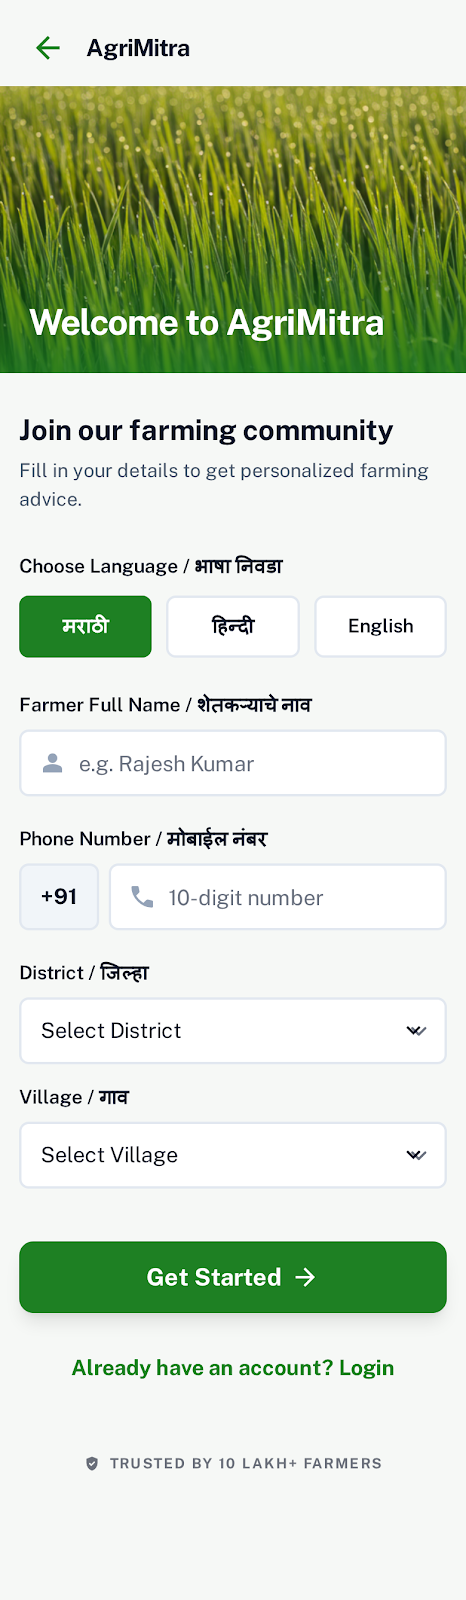
\includegraphics[width=\textwidth]{Images/screen_registration.png}
        \caption{Registration and language selection.}
        \label{fig:screen_reg}
    \end{subfigure}
    \hfill
    \begin{subfigure}[b]{0.30\textwidth}
        \centering
        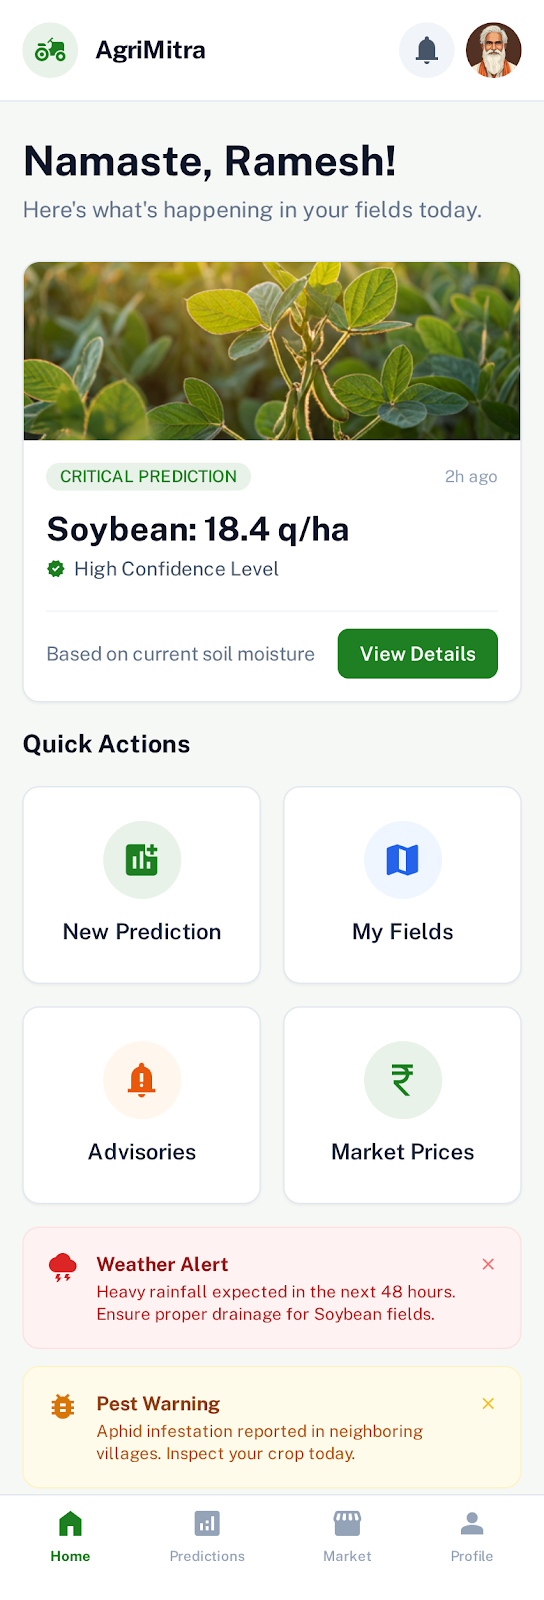
\includegraphics[width=\textwidth]{Images/screen_home.png}
        \caption{Home dashboard with last prediction and quick actions.}
        \label{fig:screen_home}
    \end{subfigure}
    \hfill
    \begin{subfigure}[b]{0.30\textwidth}
        \centering
        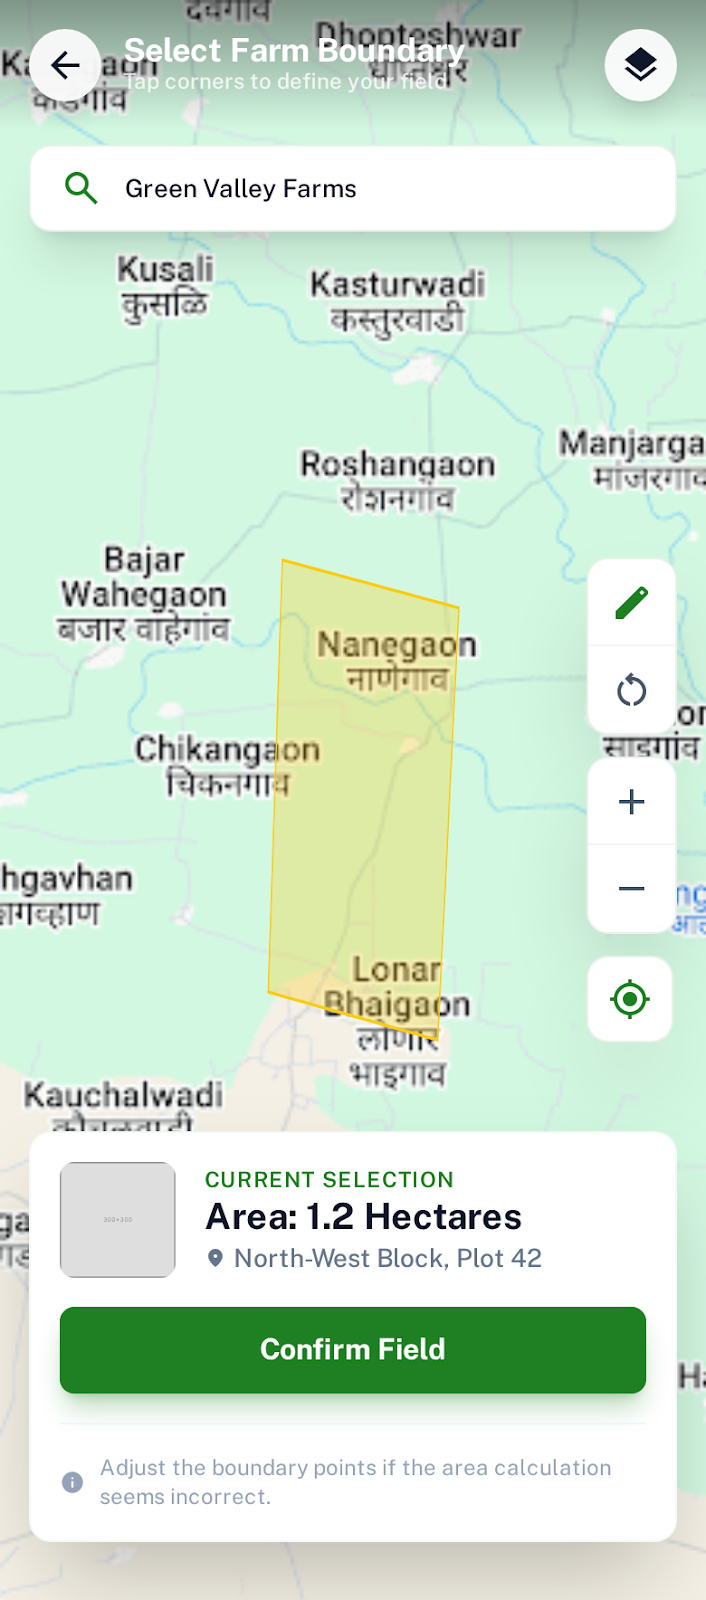
\includegraphics[width=\textwidth]{Images/screen_farm_select.png}
        \caption{Interactive farm boundary selection on satellite map.}
        \label{fig:screen_map}
    \end{subfigure}
    \caption{AgriMitra mobile application --- onboarding and farm selection screens.}
    \label{fig:screens_onboarding}
\end{figure}

\begin{figure}[H]
    \centering
    \begin{subfigure}[b]{0.30\textwidth}
        \centering
        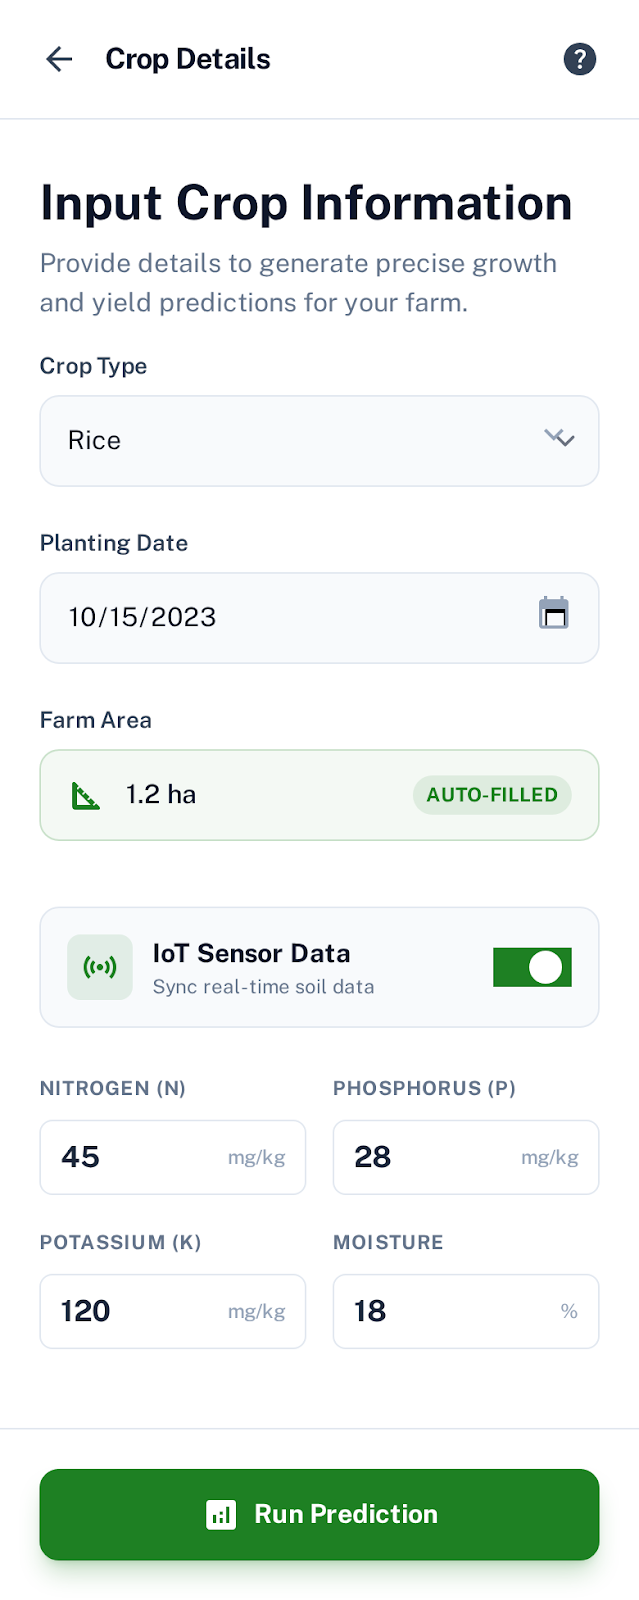
\includegraphics[width=\textwidth]{Images/screen_crop_input.png}
        \caption{Crop details and optional IoT sensor data entry.}
        \label{fig:screen_crop}
    \end{subfigure}
    \hfill
    \begin{subfigure}[b]{0.30\textwidth}
        \centering
        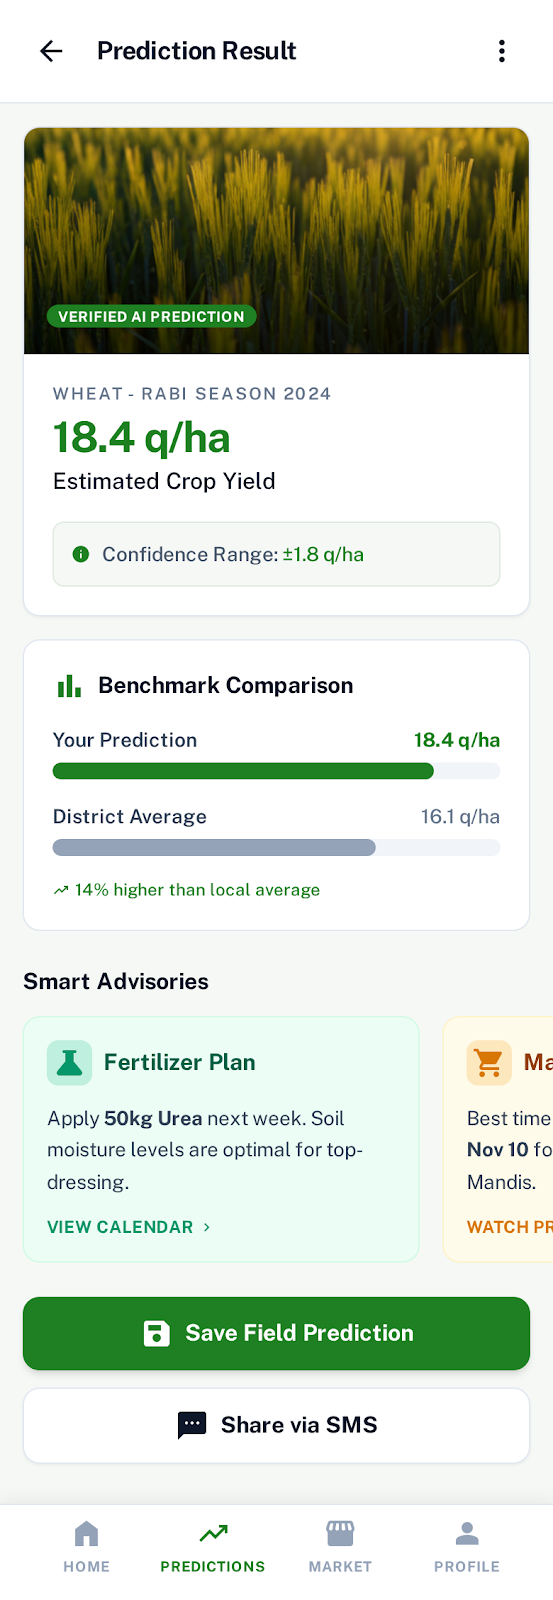
\includegraphics[width=\textwidth]{Images/screen_prediction_result.png}
        \caption{Prediction result with yield estimate and smart advisories.}
        \label{fig:screen_result}
    \end{subfigure}
    \hfill
    \begin{subfigure}[b]{0.30\textwidth}
        \centering
        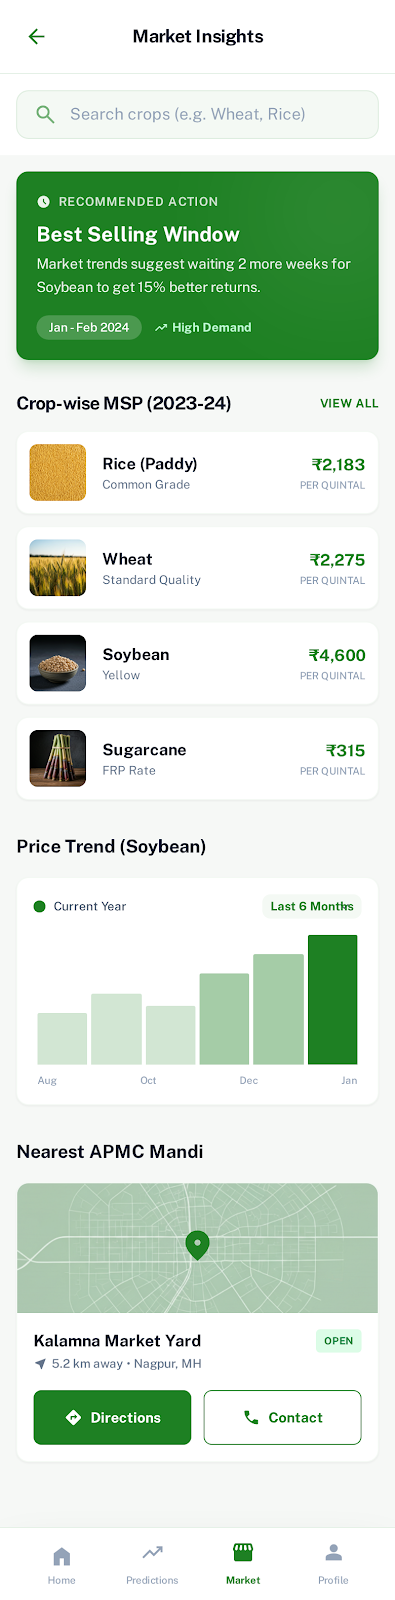
\includegraphics[width=\textwidth]{Images/screen_market.png}
        \caption{Market insights showing MSP rates, price trends, and nearest mandi.}
        \label{fig:screen_market}
    \end{subfigure}
    \caption{AgriMitra mobile application --- prediction, advisory, and market screens.}
    \label{fig:screens_prediction}
\end{figure}

